% This example An LaTeX document showing how to use the l3proj class to
% write your report. Use pdflatex and bibtex to process the file, creating 
% a PDF file as output (there is no need to use dvips when using pdflatex).

% Modified 

\documentclass{l3proj}
\usepackage{algorithm2e}
\usepackage{graphicx}
\begin{document}
\title{Project Title}
\author{Michael Kilian -- 1003819K \\
        Tony Lau -- 1102266L\\
        Dan Tomosoiu --1102486T \\
        Hector Grebbell -- 1007414G \\
        Peeranat Fupongsiripan -- 2056647F}
\date{19 March 2013}
\maketitle
\begin{abstract}

The abstract goes here

\end{abstract}
\educationalconsent
\tableofcontents
%==============================================================================
\chapter{Introduction}
\label{intro}

\input{../Intro/organisation}

%ALICE \cite{Alice} was beginning to get very tired of sitting by her sister
%on the bank and of having nothing to do: once or twice she had peeped into
%the book her sister was reading, but it had no pictures or conversations in
%it, ``and what is the use of a book,'' thought Alice, ``without pictures or
%conversations?'' \cite{Dijkstra}
%\begin{figure}
\begin{center}
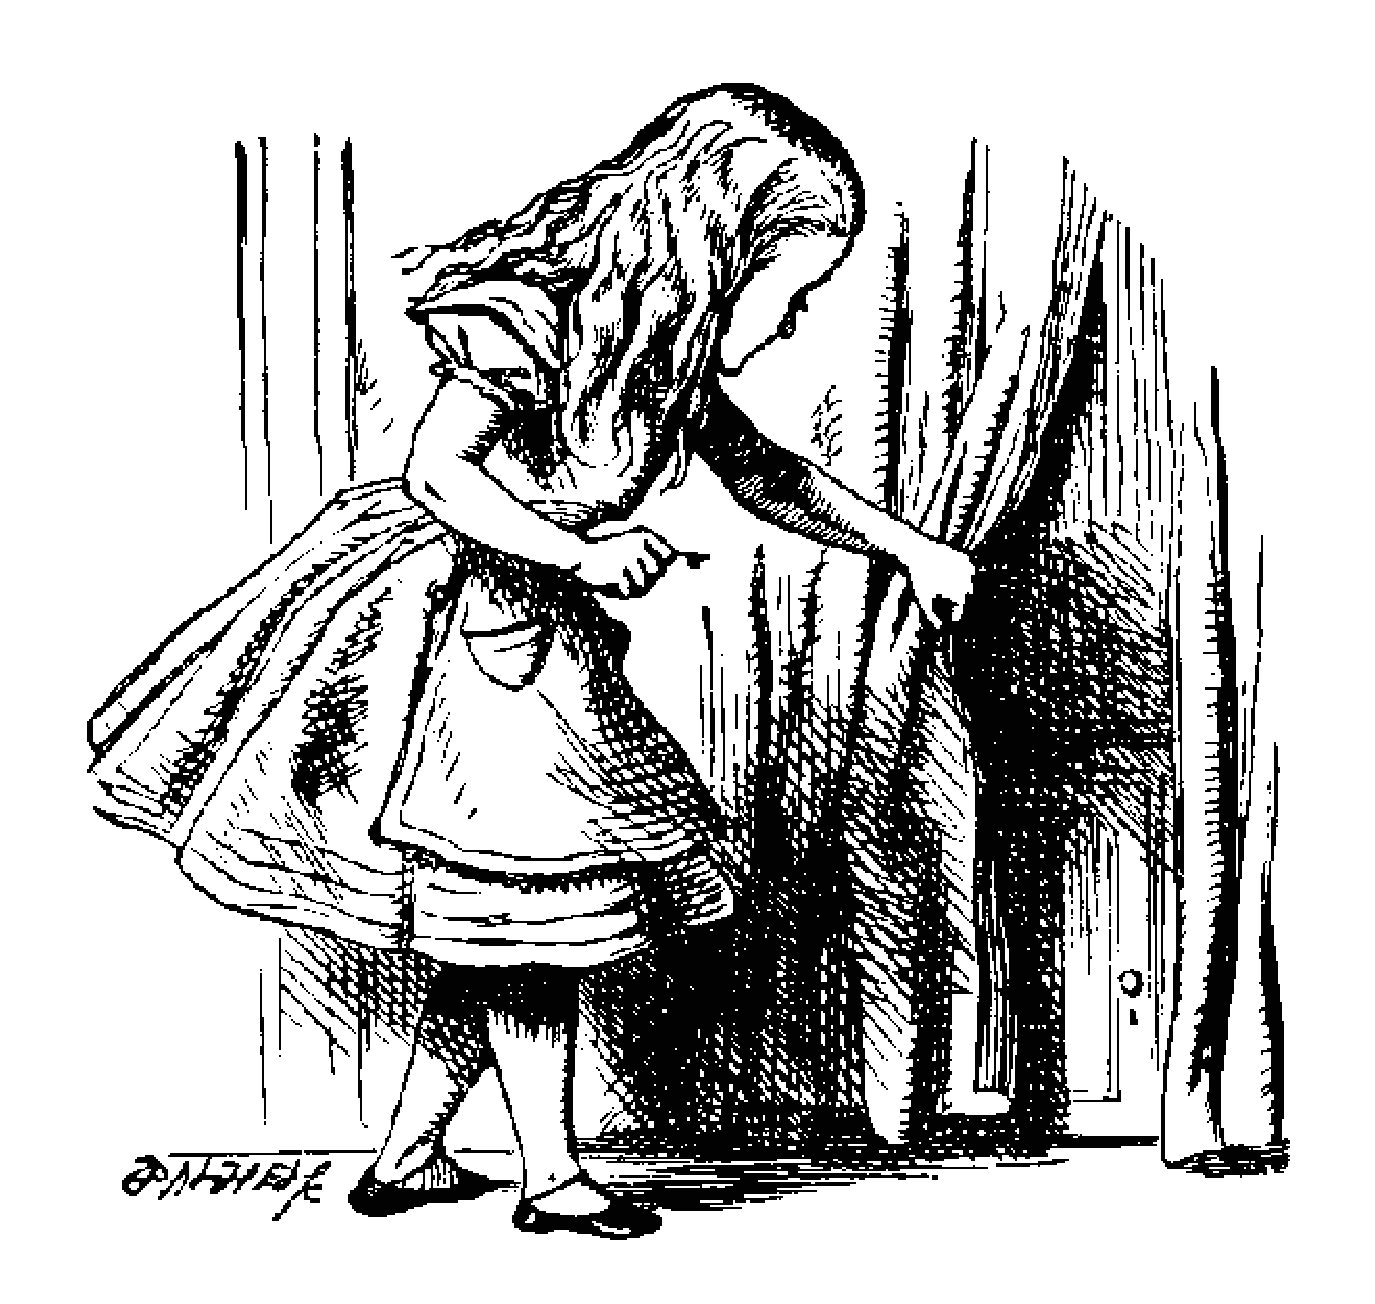
\includegraphics[width=7cm]{figures/alice}
\end{center}
\caption{Behind it was a little door}
\label{fig:alice}
\end{figure}
%Alice opened the door and found that it led into a small passage.


%==============================================================================
\chapter{Research}
\label{research}

\documentclass[a4paper,11pt]{article}
\usepackage[T1]{fontenc}
\usepackage[utf8]{inputenc}
\usepackage{lmodern}

\title{}
\author{}

\begin{document}
\section{Research into Human Behaviour}
\subsection{Non-adaptive Behaviour}
Adaptive behaviour is any behaviour is any behaviour ``which contributes directly or indirectly to an individuals survival''.
Conversely non-adaptive behaviour is any behaviour which may be counter productive to an individuals survival \cite{AdaptiveBehaviourWiki}.
In the context of an evacuation this refers to high risk actions which occur in a crowd such as stampede, pushing and shoving others,
trampling others, etc.\\
The introduction of non-adaptive behaviour can be connected to the stress a person is feeling. More specifically, Law et al \cite{CIFEResearchProposal} propose that there are three factors which contribute to the emergence of adaptive or non-adaptive behaviour:
\begin{itemize}
  \item{\textbf{Panic}: when a person perceives danger they are more likely to make irrational decisions based on instinct \cite{PanMASSEgressThesis}.}
  \item{\textbf{Decision-making}: although panicked, a person is still capable of making rational decisions. This increases the likelihood of the individual making adaptive choices, such as correctly recognising an exit or refraining from shoving upon exiting.}
  \item{\textbf{Levels of urgency to exit}: individuals within a group will experience varying levels of arguing to leave the environment based on the level of danger they perceive themselves to be in. High urgency causes individuals to behave aggresively and prioritise self-preservation.}
\end{itemize}
All of these theories provide insights into human behaviour but have yet to be unified into a comprehensive theory.

\subsection{Bounded Rationality}
\label{subsec:boundedRationality}
Bounded Rationality can be expressed as the principle that in a given situation the rational decisions a person can make are bounded by the set of possible options available to them and the time in which they can make a decision. This concept was initially proposed by Herbert Simon, who highlighted two interlocking components of bounded rationality \cite{BoundedRationalityDefinition}:
\begin{itemize}
  \item{\textbf{The limitations of the human mind}: the human mind does not have limitless processing power or memory and so must use approximate methods to handle most tasks. For computational purposes these methods can be expressed using simple heuristics.}
  \item{\textbf{Environmental structure}: Simon emphasised that the heuristics used must be adapted to the environment in which the decision is made.}
\end{itemize}
An important example of this priciple is Simon's concept of satisficing: a ``method for making a choice from a set of alternatives encountered sequentially when one does not know much about the possibilities ahead of time'' \cite{BoundedRationalityDefinition}. In an evacuation a person will use this satisficing technique to make decisions such as where to move next based on what they can see.\\
It is important to note that, like other rational behaviours, this process can be disrupted by the introduction of stress factors, as previously discussed.

\subsection{Conformity \& Social Proof Theory}
\label{subsec:socialProof}
Conformity can be defined as a "change in behaviour or belief toward a group as a result of real or imagined group pressure". This can be further divided into \emph{normative influence} and \emph{informational influence}. Normative influence refers to changes in behaviour for the sake of winning the approval of other group members. Informational influence refers to conforming in an attempt to improve one's knowledge of reality and current situation. \cite{HandbookOfPsychology5}.\\
Informational influence, which is often called Social Proof Theory \cite{SocialProofWiki},  has the effect that when facing a situation with uncertainty, a person may turn to the surrounding group for cues. Cialdini noted ``we seem to assume that if a lot of people are doing the same thing, they must know something we don't'' \cite{PanMASSEgressThesis}.\\
This principle is at the core of many of the behaviours observed in evacuations, particularly herding behaviour \cite{PanMASSEgressThesis,MultiAgentFramework}.

\subsection{Personal Space}
\label{subsec:personalSpace}
According to Edward T. Hall \cite{HiddenDimension} the space surrounding a person can be divided into four ``reaction bubbles'' which represent an acceptable radius around the person in which different categories of interaction. These are:
\begin{itemize}
  \item{\textbf{Public Space}: this space is used for speeches or other interactions with large audiences. This includes anything beyond roughly 2.4m}
  \item{\textbf{Social Space}: the distance reserved for interaction with strangers or newly formed groups. This ranges from around 1.2m to 2.4m}
  \item{\textbf{Personal Space}: this begins an arms length away from the individual's center and is reserved for interactions with friends or other close associates}
  \item{\textbf{Intimate Space}: The smallest of the spaces, this ranges from touching the person to around 50cm from their body. Interactions in this space are extremely personal and normally occur only with close members of family or friends}
\end{itemize}
The last two of these spaces are of particular interest. Another definition of personal space is the area surrounding an individual ``into which others may not intrude without causing discomfort'' \cite[pg. 424]{HandbookOfPsychology5}.\\
In a crowded environment the violation of ones personal space is likely to increase stress and anxiety (see page \pageref{subsec:personalSpace}. Naturally this effect is even greater when the intimate space is violated. An individuals desire to re-establish this boundary can introduce non-adaptive behaviour.\\
It should be noted that the definition of these four spaces varies between individuals and between different cultures. Therefore the ranges discussed here are only an estimate \cite{ProxemicsWiki}. \ref{fig:personalSpace} shows these `bubbles'.

\begin{figure}
\centering
\includegraphics{Images/PersonalSpace.png}
\caption{Edward T Hall's `reaction bubbles'}
\label{fig:personalSpace}
\end{figure}


\subsection{Classes of Evacuation Behaviour}
The MASSEgress framework \cite{MultiAgentFramework,PanMASSEgressThesis,IndivBehaviourPseudo} defines three classes of evacuation behaviour which will be considered in this projects behavioural model for agents. These are \emph{competitive behaviour}, \emph{queueing} and \emph{herding}.
\subsubsection{Competitive Behaviour}
Competitive behaviour is observed when individuals attempt to force their own exit by competing with others. This includes pushing, moving at an unsafe speed towards exits, etc. Such behaviour generally reduces the efficiency of egress, especially at narrow doorways or other tight spaces\cite{BottleneckStudy}, compared to exiting in a non-competitive (queuing) manner \cite{EgressBehaviourKirchner}.\\
In general this behaviour emerges when a person is highly stressed and perceives an urgent need to evacuate. However an individual can also take up competitive behaviour as a result of social proof, if other individuals around them are acting competitively.
\subsubsection{Queueing}
This can be seen as the converse of competitive behaviour. It is characterised by a group organising themselves to facilitate efficient and safe passage through an exit.
\subsubsection{Herding}
Broadly speaking one can define herding as "the alignment of the thoughts or behaviours of individuals in a group (herd) through local interaction and without centralized coordination" \cite{HerdingInHumans}. Again social proof is a key contributor to the emergence of this behaviour. When an individual has a high degree of uncertainty they will follow the crowd.\\
Unlike other behaviours herding can be either adaptive or non-adaptive depending on the context in which it occurs. Suppose that an individual is following a crowd through an exit. It is possible that this exit is the correct way to proceed, so this choice has aided the person's egress. Equally it may lead to a dead end.

\subsection{Unifying These Concepts In A Behavioural Model}
We have discussed some of the properties of an individual and groups (such as panic, urgency to exit, etc.) which affect the behaviours exhibited in the evacuation process.\\
For modelling purposes, these factors are unified into a single parameter which shall be referred to as `evacuation stress'. This can be expressed as a percentage where 0 is equivalent to an individual being in regular day-to-day conditions, whereas 100 represents an individual in blind panic acting almost entirely on instinct. Of course these two extremes are unlikely to occur in practice.\\
The reason for this extreme simplification is to limit the possible conditions which must be checked in decision making. The more attributes an agent possesses which may affect decision making there are, the more conditions must be checked at each decision making stage. Even a small number of variables can lead to an very large set of possible outcomes which all must be checked. This can exponentially increase both the complexity of the behavioural model for the programmer and the computational complexity of making a decision.
\subsection{The Perceive, Decide, Act Process}
The decision making process for each agent can be expressed in three stages:
\begin{enumerate}
  \item{\textbf{Perceive}: the agent scans the area around themselves for visible goals or other information. This produces a set of goals in sight.}
  \item{\textbf{Decide}: based on what they can perceive and their current level of evacuation stress, the agent chooses an action with which to proceed.}
  \item{\textbf{Act}: the agent carries out this action.}
\end{enumerate}
An example of this procedure is as follows:
\begin{enumerate}
  \item{An agent scans the room they are in. They perceive two exits, one with only two people moving through it, the other with twenty people waiting at it.}
  \item{The agents current evacuation stress is high enough that they will engage in herding behaviour. They decide to move toward the most crowded of the two doors.}
  \item{The agent plans their route to this destination and initiates the movement.}
\end{enumerate}
 The implementation of this theory is discussed in the Implementation section.
\bibliographystyle{unsrt}
\bibliography{references}
\end{document}


%Requirements (chapter on its own?)

%------------------------------------------------------------------------------

%==============================================================================
\chapter{Design}
\label{design}

\input{../Design/PopulationandGoalDesign}

%The following diagrams (especially figure \ref{fig:alice}) illustrate the process...

%==============================================================================
\chapter{Implementation}
\label{impl}

%In this chapter, we describe how the implemented the system.

%\documentclass{article}
%\usepackage{algorithm2e}
%\begin{document}
\section{Route Planning}
\label{Imp:sec:routePlanning}
Planning an agent's route from its current point to a given point is acheived by a collaboration between a Person and PersonNavmeshRoutePlanner instance. Routes are stored using the jMonkeyEngine class MotionPath. This contains a set of waypoints and methods to animate the agent's movement between these waypoints. The maximum distance between each waypoint is roughly constant and can be set as a parameter to the following procedure (it is not constant when the agent must turn at a point closer to its current position that the maximum distance between points). The distance used is an important decision in the implementation. If it is too large the accuracy of the animation tends to degrade. If it is too low then a large number of waypoints will be stored needlessly. After extensive experimentation 0.5 was found to be an acceptable value for the maximum distance between waypoints. In practice this provided a balance between quality and efficiency.\\
A route is calculated in two stages:
\begin{enumerate}
\item{A path is calculated on the navigation mesh using a modified A* algorithm to traverse the mesh like a graph. This returns a small set of points. These points illustrate the lines of motion an agent must take to reach their goal. This is performed in the constructor for a PersonNavmeshRoutePlanner.}
\item{Using these points as guidance, the path is `fleshed out' by moving along the path and placing MotionPath waypoints no further apart than the defined maximum
distance. This terminates with a waypoint being placed on the goal location the agent must reach.}
\end{enumerate}
Note that a fresh PersonNavmeshRoutePlanner instance must be instantiated to calculate a route. The relationship between the Person and PersonNavmeshRoutePlanner instances is expressed in \ref{fig:RoutePlanSequence}.

\begin{figure}
\label{fig:RoutePlanSequence}
\centering
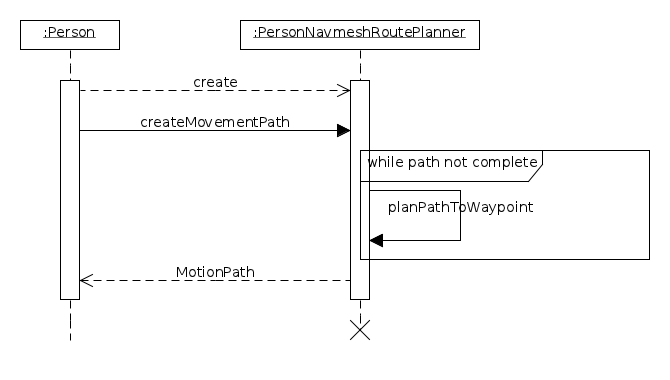
\includegraphics[scale=0.5]{../UMLDiagrams/RoutePlanningSequence.png}
\caption{Generation of an agent route as a MotionPath}
\end{figure}


\section{Implementing the Perceive, Decide, Act Process}
\label{Imp:sec:perceiveDecideAct}
Here we discuss the techniques and algorithms used to realise the Perceive, Decide, Act process previously discussed in Section \ref{Res:subsec:perceiveDecideAct}.

%%%%%%%%%%%%%%%%%%%%%%%%%Perception Implementation
\subsection{Perception}
\label{Imp:subsec:perception}
Agent perception is achieved using the following simple algorithm:

\begin{algorithm}[H] %%%%%%%Agent Perception Algorithms
 \SetAlgoLined
 \SetKwInOut{Input}{input}
 \SetKwInOut{Output}{output}
 \Input{The set of goals in the environment: \emph{goals}}
 \Output{A set of goals visible to the user at the given instant in time: \emph{visibleGoals}}
 \BlankLine
 \For{each goal g in goals}{
  \If{g is in line of sight of agent}{
    add g to visibleGoals\;
  }
  }
  \caption{Agent Perception Algorithm}
\end{algorithm}

%%%%%%%%%%%%%%%%%%%%%%%%%%%%%Decision Implementation
\subsection{Decision}
\label{Imp:subsec:decision}
In the Research Chapter [Reference] the three classes of human behaviour considered in the scope of this project were defined. In practice, only herding behaviour implemented as part of the Decide step; queueing and competetive behaviour must be handled asynchronously using collision avoidance techniques. Unfortunately collison avoidance was not implemented in the final system due to various problems discussed in Section \ref{Problems:subsec:problemsecountered}. Future solutions to implement collision avoidance are discussed in Section \ref{Problems:subsubsec:ORCA}.
To decide on a new action, an agent must select one of the visible goals that were found in the Perceive step (if any). Otherwise it must continue on its current path. The decision making process is realised using an extendable algorithm, which sequentially considers sets of different classes of goal according to their priority. Exits have the highest priority.\\

The final algorithm only makes decisions regarding exits, due to various issues which emerged during development (see Section \ref{Problems:subsec:problemsecountered}). However it is easy to extend this process to include other goal types by adding further conditionals following the pattern laid out below.\\

%%%%%%%%%%%%%%%%%%%%%%%%%%%Decide Algorithm
\begin{algorithm}[H]
 \SetAlgoLined
 \SetKwInOut{Input}{input}
 \SetKwInOut{Output}{output}
 \Input{Person person, ExitGoal[ ] exits /*add further exit types here as arrays */}
 \Output{Target Goal for agent to move toward}
 \eIf{no of exits $>$ 0}{
   ExitGoal \emph{currentExit} = $exits[0]$\;
   \eIf{person is stressed}{
     \For{each exit \emph{e} in exits}{
       \If{number of people queuing at e $>$ no. of people queueing at targetExit}{
	targetExit = e\;
	}
      }
    return targetExit\;
    }{ %%%%%%%%%%%inner else
     Vector3f position = person.location\;
     \For{each exit e in exits}{
       \If{distance to e $<$ distance to targetExit}{
	targetExit = e\;
	}
      }
      return targetExit\;
     }
}{ %%%%%%%%outer else
  return null;
}
\end{algorithm}

\subsection{Act}
\label{Imp:subsec:act}
This step's representation in the BehaviouralModel class is trivial since the Decide step already returns a target goal. It is left in as a place for performing any calculations which should be performed before returning the target goal to the agent.\\
Upon receiving a new target goal, an agent should perform the following:
\begin{itemize}
\item{Use a PersonNavmeshRoutePlanner to calculate a route to this goal}
\item{Set the returned MotionPath as the current MotionPath for the agent}
\item{Begin moving down this path}
\end{itemize}




%\end{document}
     
     
 

    



%------------------------------------------------------------------------------
\section{User Interface}

Blah blah blah
Blah blah blah
Blah blah blah
Blah blah blah

% - - - - - - - - - - - - - - - - - - - - - - - - - - - - - - - - - - - - - - -
\subsection{Foo}

Blah blah blah
Blah blah blah
Blah blah blah
Blah blah blah

%------------------------------------------------------------------------------
\section{Database Model}

\begin{enumerate}
\item Blah blah blah
\item Blah blah blah
\item Blah blah blah
\item Blah blah blah
\end{enumerate}



%==============================================================================
\chapter{Evaluation}

% This example An LaTeX document showing how to use the l3proj class to
% write your report. Use pdflatex and bibtex to process the file, creating 
% a PDF file as output (there is no need to use dvips when using pdflatex).

% Modified 

%\documentclass{article}
%\begin{document}
%\title{User Interface Evaluation}
%\author{Tony Lau}
%\maketitle
%==============================================================================
\section{User Interface Evaluation Methods}
\label{evalmethods}

The simulator will be evaluated through a series of user tests with different participants. The goals of the user interface evaluation are to assess the effect of the interface on the user and to identify specific problems which should be rectified. The simulator will be first tested with the fire warden of The Tall Ship who is the primary user of the system. Secondly, feedback on usability of the system will be gathered from usability testing with the subjects being students at the University of Glasgow.

Two evaluation methods, namely Heuristic Evaluation and Usability Experiments, will be used to determine whether the requirements specified in section \ref{requirements} have been met and also to determine the overall usability of the system.

\subsection{Heuristic Evaluation}
Heuristic evaluation is a usability inspection method pioneered by Jakob Nielsen and Rolf Molich which helps to identify problems with a user interface by judging the interface's compliance to recognized usability principles -- heuristics\cite{heuristics}.

The heuristics made use of in this part of the evaluation are Nielsen's Heuristics, developed by Jakob Nielsen and Rolf Molich in 1990\cite{tenheuristics}. Nielsen refined the original set of heuristics in 1994\cite{tenheuristics}. Below is list of the heuristics and a description of each one:
\\
\textbf{1. Visibility of system status:}
The system should always keep users informed about what is going on, through appropriate feedback within reasonable time.
\\
\textbf{2. Match between system and the real world:}
The system should speak the user's language, with words, phrases and concepts familiar to the user, rather than system-oriented terms. Follow real-world conventions, making information appear in a natural and logical order.
\\
\textbf{3. User control and freedom:}
Users often choose system functions by mistake and will need a clearly marked "emergency exit" to leave the unwanted state without having to go through an extended dialogue. Support undo and redo.
\\
\textbf{4. Consistency and standards:}
Users should not have to wonder whether different words, situations, or actions mean the same thing. Follow platform conventions.
\\
\textbf{5. Error prevention:}
Even better than good error messages is a careful design which prevents a problem from occurring in the first place. Either eliminate error-prone conditions or check for them and present users with a confirmation option before they commit to the action.
\\
\textbf{6. Recognition rather than recall:}
Minimize the user's memory load by making objects, actions, and options visible. The user should not have to remember information from one part of the dialogue to another. Instructions for use of the system should be visible or easily retrievable whenever appropriate.
\\
\textbf{7. Flexibility and efficiency of use:}
Accelerators -- unseen by the novice user -- may often speed up the interaction for the expert user such that the system can cater to both inexperienced and experienced users. Allow users to tailor frequent actions.
\\
\textbf{8. Aesthetic and minimalist design:}
Dialogues should not contain information which is irrelevant or rarely needed. Every extra unit of information in a dialogue competes with the relevant units of information and diminishes their relative visibility.
\\
\textbf{9. Help users recognize, diagnose, and recover from errors:}
Error messages should be expressed in plain language (no codes), precisely indicate the problem, and constructively suggest a solution.
\\
\textbf{10. Help and documentation:}
Even though it is better if the system can be used without documentation, it may be necessary to provide help and documentation. Any such information should be easy to search, focused on the user's task, list concrete steps to be carried out, and not be too large.\\

The user interface of the simulator will be examined and evaluated using the descriptions of each of Nielsen's 10 Heuristics above. Heuristic Evaluation is a relatively quick and inexpensive way to evaluate a user interface. Deviation from recognized usability principles, identified from the evaluation, can provide great insight into how the user interface could be further refined to enhance the usability of the system.

\subsection{Usability Experiments}
Usability experiments can be used in addition to Heuristic Evaluation to gain further feedback on the system. These are particularly useful because they allow the experimenter to gain insight to the reactions of the users of the system first-hand.

Two different sets of users will be used for evaluation: the Tall Ship's fire warden and a group of students. The fire warden will be able to tell us whether the system meets the requirements and also on how usable the system is. Since it is unlikely that the students work in the domain of fire safety, the set of students will be primarily used to test the ease in which the system can be used. Any suggestions of improvements to the system by either group will also be recorded.

\subsubsection{Experimental Design}
The experiment must be designed carefully in order to provide results that are both reliable and generalisable. Two types of experimental design can be used: within-subjects design and between-subjects design.

In a between-subjects (or randomized) design, each participant is given a different condition, of which there are at least two. A control condition, where the independent variables are not changed, is needed to ensure the measured differences in the other conditions are true. Since each subject only performs under one condition, the likelihood of any learning effect from performing two similar conditions one after the other is mitigated. However, a between-subjects design requires a large number of participants if one is going to extract meaningful information.

In a within-subjects design, each subject is given the same conditions to perform. The effect of learning is more prominent in this method, which is a disadvantage but it has an advantage compared to between-subjects design because less subjects and time are required.

Considering the advantages and disadvantages of both methods, a within-subjects design will be adopted for the user interface evaluation of the evacuation simulator. Since limited resources are available in terms of time and users, the less costly within-subjects design is more appropriate. Learning effects can be lessened by changing the order in which the conditions are carried out by the participants. This allows a comparison of participants who carried out a condition first and participants who carried out the condition after another one, and therefore subject to learning. The results from the within-subjects evaluation will be analysed to determine whether effects of learning have adversely affected the results of the evaluation.

For both sets of users, they will carry out a set of fixed tasks and the time taken to perform these tasks as well as any mistakes they make will be recorded. This data will be used to form the evaluation results and will allow the identification of flaws in the usability of the system and areas for improvement.

\subsubsection{Think-aloud Protocol}
In addition to the usability experiment discussed above, the think-aloud protocol will also be used to gather information from users of the system. This method was introduced in the usability field by Clayton Lewis and is discussed in Task-Centered User Interface Design: A Practical Introduction by C. Lewis and J. Rieman\cite{uidesign}. Think-aloud protocols involve participants thinking aloud as they perform a set of pre-specified tasks. The idea is to have the users of the system saying out loud exactly what they are doing and how they are feeling. This allows the experimenter to gain a first-hand sight of a user using the product and provides insightful knowledge into how the end user would go about performing tasks.

The information gathered from the experiment will be analysed and the difficulties the user had will be discussed and rectified by changing the user interface. Any major changes to the user interface will have to be evaluated again to ensure the changes actually improve the usability of the system as a whole. 

\subsection{NASA TLX: Task Load Index}
%\begin{itemize}
%\item NASA TLX was used after the Think Aloud evaluation to measure the workload of the participants relating to the tasks that they had just performed. Talk about what it is and how it measures workload.
%\item Include pictures of the rating scale and the description of the rating scale from the instruction manual.
%\item Discuss the pairwise comparison and whether to use Raw TLX (RTLX). Cite 20 years later paper.
%\end{itemize}

NASA Task Load Index (TLX) will be used to measure the workload of the participants relating to the tasks that they are asked to perform. It is a subjective workload assessment tool which is used to derive an overall workload score based on a weighted average of the six subscales, namely Mental Demands, Physical Demands, Temporal Demands, Own Performance, Effort and Frustration\cite{tlx}.

\begin{figure}[H]
	\centering
	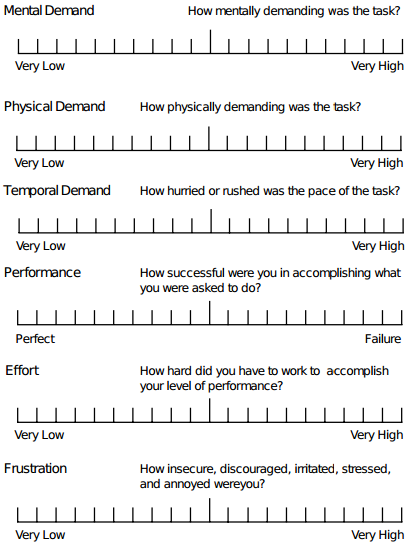
\includegraphics[scale=0.4]{../images/ratingscale.png}
	\caption{NASA TLX Rating Scales}
\end{figure}

After the participants have given a rating on each of the six subscales, they are asked to carry out a pairwise comparison between the subscales to identify their relative importance, in the eyes of the user.

This particular experiment involves asking the user to carry out pairwise comparisons, however, some research has suggested that the exclusion of the pairwise comparisons between subscales can increase experimental validity\cite{tlxinvariance}.

%==============================================================================================
\section{User Interface Evaluation Results}
\label{results}

The results from the user interface evaluation using heuristic evaluation, think-aloud and NASA Task Load Index (TLX) are discussed below.

\subsection{Heuristic Evaluation}
\subsubsection{Visibility of system status}
The system gives users little information about what is going on. For example, on pressing the populate or route buttons, no information is displayed on the screen informing the user that something is happening in the background. As a result, the user could be left wondering whether the button was correctly clicked.

Inclusion of messages on the screen stating what is happening at a particular moment in time would help the users to identify the status of the system. For example, inclusion of a message saying that the system is loading instead of a black screen will inform the user that something is indeed happening. Messages when the user clicks a button confirming that the action is happening and a message that displays on the screen when the evacuation simulation has finished will also increase the user’s awareness of the system status which in turn makes the system more user friendly.

\subsubsection{Match between system and real world}
The arrow keys (up, down, left and right) for camera movement are positioned in a logical order which would be familiar to the majority of users. This allows an easy mapping from real world natural conventions to the system which makes the system easier to use. Non-natural placement of these buttons on the screen would cause confusion in users and lead to frustration.

The system does use the term `navmesh' in the checkbox labelled `show navmesh'. The user is likely to be unfamiliar with this technical term and would thus have to consult the documentation to learn properly what it does. The system should use words and phrases familiar to the user so it would seem appropriate to replace the word `navmesh' with something along the lines of `ship outline' or `wireframe'.

\subsubsection{User control and freedom}
The user has the ability to control the camera manually using the on-screen buttons. The allows the user to view the ship in any way they want. There is also functionality to increase or decrease the speed of the camera and also to select preset camera locations from a drop-down menu which increases the control and freedom the user has. The number of preset camera locations is currently two. This should be expanded to give the user more options.

The user can change the population size from the main screen and a more advanced settings menu allows the user to create categories of people according to various factors. This gives advanced users more freedom in the interactions they make with the system.

\subsubsection{Consistency and standards}
In general, the buttons are labelled well and the user does have to wonder what they do. However, some problems exist in the camera settings part of the main screen. There are two up arrows and two down arrows and their functionality is not made entirely clear to the user. One of the up arrows is to pan up and the other up arrow is to rotate upwards. This should be made clear to the user by either increasing the size of the button and including a meaningful button name, or include the information as text above the buttons on the camera controls panel itself.

\subsubsection{Error prevention}
Some steps have been taken to prevent the users from executing an action which would lead to an error in the system. The evacuate button is grayed out and is only allowed to be clicked by the user when the ship has been successfully populated. By stopping the user from performing this action until it is appropriate, allows the prevention of an illegal system state -- namely evacuating an empty ship.

Error prevention related to the other buttons was overlooked and should be corrected. Other buttons on the main panel of the user interface should also be grayed out when it would not be appropriate to click.

Where there exist fields which can be altered by the user (for example, the population size field) a maximum and minimum value has been defined to prevent the user from entering too high or too low a number. This eliminates the possibility that the system will enter a state which it cannot handle as a result of user input which protects the system from mistakes made by the user.

\subsubsection{Recognition rather than recall}
The main buttons on the user interface are made to be as self explanatory as possible, however one shortfall is the design of the camera location panel. As discussed in the consistency heuristic, it should be made more clear what these buttons actually do. This would remove the need of the user to consult documentation for help and would thus reduce the extent of recall from one dialog to the next.

\subsubsection{Flexibility and efficiency of use}
The system has the ability to cater for more experienced user as mentioned in the user control and freedom heuristic. There exists the ability for the more experienced user to change a variety of properties of the camera such as speed and location. There is also the ability to use the keyboard to navigate around the ship which would allow more experienced users to increase their speed of interaction with the system.

There is, however, no method of allowing the user to tailor frequent actions through the use of accelerators or custom keyboard shortcuts, for example. The addition of such features would increase development time and since the experienced users group is a minority, it would not be in the best interest to develop this feature at this time.

\subsubsection{Aesthetic and minimalist design}
The system has a main screen which includes the most often used actions, and a settings screen which includes extra functionality. This separation allows a less cluttered minimalist view in the main screen which is easier to comprehend for the user. The system had been designed to display elements positioned in a natural way, allowing the user to focus on using the system and not needing to familiarise themselves with the interface for too long.   

\subsubsection{Help users recognize, diagnose and recover from errors}
As mentioned in the prevention of errors heuristic above, some steps have been taken to prevent the user from making errors. However, since not all sections of the interface are removed from use when they are not supposed to be used, it is possible for a user to crash the system by pressing the buttons repeatedly. There are no friendly error messages to tell the user that something has went wrong -- they are presented with a black screen. This leaves the user wondering whether the system is busy in the background carrying out some task, or has crashed.

To resolve this problem, better messages should be displayed on the screen to the user to increase visibility of system status. This would eliminate any confusion from the user when using the system. A reset button should also be implemented as a last resort for the user to click if the system crashes for an undocumented reason. This will ensure robustness in the system and increase the user-friendliness as a whole.

\subsubsection{Help and documentation}
No help or documentation is provided to the user. While the majority of the system is, on the whole, quite intuitive to use, some parts such as the camera controls panel and the advanced settings dialog box would benefit from documentation.

Brief documentation on the basic parts of the interface and what each button does as well as more detailed documentation on the more complex parts of the system should be created to assist the user in using the system and making decisions.

\subsection{Think Aloud}
The Think Aloud evaluation of the user interface was carried out with eight participants. The participants were asked to complete the six tasks listed below and were encouraged to ‘think aloud’ during the evaluation. The participants were observed and notes were taken to allow a discussion of improvements which could be made to the user interface after the evaluation.
\\
\\
\textbf{Tasks}
\begin{enumerate}
\item Set the population size to 50. Populate the ship.
\item Hide the ship frame from view, then show it again.
\item Generate the exit routes for the population.
\item Change the camera angle so you have a bird's eye view of the ship.
\item Evacuate the ship. While the evacuation is taking place, change the camera view to face the exits of the ship.
\item Read out loud the time the simulation took and the number of people evacuated.
\end{enumerate}
A summary of the findings of the Think Aloud evaluation is discussed below. Detailed notes on a per-participant level are included in Appendix C.

\begin{itemize}
\item The visibility of system status was a clear shortfall as indicated by the participants. Particularly in tasks 1, 3 and 5 where buttons which required the user to wait after being pressed, the participant was left guessing whether anything was happening with the system or whether they had done something wrong.
\item The meaning of the camera location buttons was also not as clear as they should have been. Participants had to investigate what the buttons did and clear labelling would have solved this issue.
\item The participants had no difficulty identifying key information such as number of people evacuated and the time taken for the evacuation which confirms that the information is well visible and the labelling is unambiguous.
\item Identification of the completion of the evacuation was most often done by looking at whether anything more was happening in the graphical representation rather than looking at the `remaining people' metric at the right hand side of the interface. It was noted that a pop-up message when the simulation is complete would make this more clear to the user.
\item The terminology used in the user interface must be standardised to remove jargon words such as ‘navmesh’ which would be unclear to the user. Task 2 highlighted that while some users guessed that ‘ship frame’ was equivalent to the ‘navmesh’ in this particular situation, 5 of the 8 participants were confused by the technical language. 
\end{itemize}

\subsection{NASA TLX: Task Load Index}
%\begin{itemize}
%\item Insert graph.
%\item Discuss that there is a low workload in using the system.
%\end{itemize}

\begin{figure}[H]
	\centering
	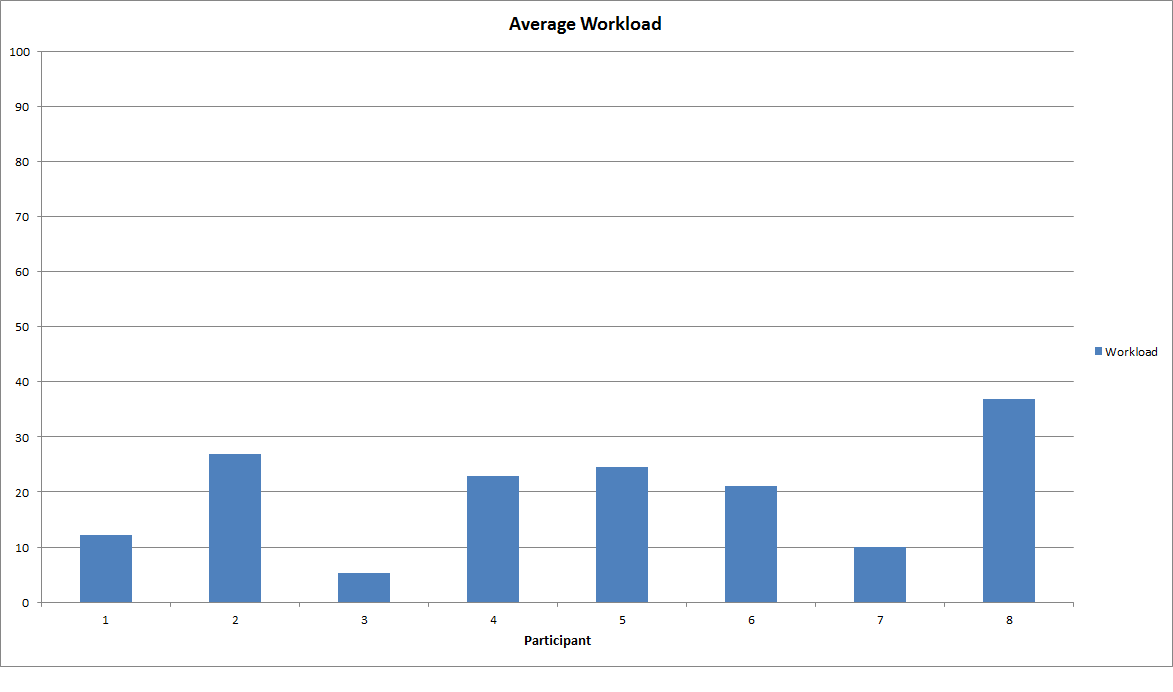
\includegraphics[scale=0.25]{../images/tlxresults.png}
	\caption{Average workload across participants}
\end{figure}

The above image shows the average workload of the eight participants in the experiment, which is calculated based on the ratings and pairwise comparisons given by the participant. It can be seen that the overall workload of each participant is reasonably low and so it can be said that using the system is not demanding. 

%==============================================================================================


%==============================================================================
%\end{document}


%==============================================================================
\chapter{Conclusion}

A great project!

%==============================================================================
\section{Contributions}

Here we explain that Lewis Carroll wrote chapter \ref{intro}. John Wayne
was out riding his horse every day and didn't do anything. Marilyn Monroe
was great at getting the requirements specification and coordinating the
writing of the report. Betty Davis did the coding of the kernel of the
project, described in Chapter \ref{impl}.  James Dean handled the
multimedia content of the project.

%==============================================================================
\bibliographystyle{plain}
\bibliography{teamL_dissertation_2013}
\end{document}
